\documentclass[conference]{IEEEtran}

\IEEEoverridecommandlockouts

\usepackage{cite}
\usepackage{amsmath,amssymb,amsfonts}
\usepackage{algorithmic}
\usepackage{graphicx}
\usepackage{textcomp}
\usepackage{float}
\usepackage[table]{xcolor}
\usepackage{array}
\usepackage{booktabs}
\usepackage{tabularx}      % Para o ambiente tabularx
\newcolumntype{C}[1]{>{\centering\arraybackslash}m{#1}}
\renewcommand{\thetable}{\Roman{table}}
\def\BibTeX{{\rm B\kern-.05em{\sc i\kern-.025em b}\kern-.08em
    T\kern-.1667em\lower.7ex\hbox{E}\kern-.125emX}}

\begin{document}

\title{Sistema de Apoio à Manutenção Preditiva Baseado na Análise de Vibração *\\
{\footnotesize \textsuperscript{*}Note: Sub-titles are not captured for https://ieeexplore.ieee.org  and
should not be used}
\thanks{Identify applicable funding agency here. If none, delete this.}
}

\author{\IEEEauthorblockN{1\textsuperscript{st} Gabriel Macedo Lemos}
\IEEEauthorblockA{\textit{Instituto Federal Sul Rio Grandense} \\
Pelotas, Brasil \\
gabrielmlemos30@gmail}
\and
\IEEEauthorblockN{2\textsuperscript{nd} Given Name Surname}
\IEEEauthorblockA{\textit{dept. name of organization (of Aff.)} \\
\textit{name of organization (of Aff.)}\\
City, Country \\
email address or ORCID}
}

\maketitle

\begin{abstract}
This document is a model and instructions for \LaTeX.
This and the IEEEtran.cls file define the components of your paper [title, text, heads, etc.]. *CRITICAL: Do Not Use Symbols, Special Characters, Footnotes, 
or Math in Paper Title or Abstract.
\end{abstract}

\begin{IEEEkeywords}
component, formatting, style, styling, insert.
\end{IEEEkeywords}

\section{Introduction}
Fazer depois.

\subsection{Maintaining the Integrity of the Specifications}

The IEEEtran class file is used to format your paper and style the text. All margins, 
column widths, line spaces, and text fonts are prescribed; please do not 
alter them. You may note peculiarities. For example, the head margin
measures proportionately more than is customary. This measurement 
and others are deliberate, using specifications that anticipate your paper 
as one part of the entire proceedings, and not as an independent document. 
Please do not revise any of the current designations.

\section{Fundamentação Teórica}
Com o avanço tecnológico e as sucessivas revoluções
industriais, houve um crescente investimento e valorização da manutenção, uma vez que
paradas não planejadas resultam em prejuízos econômicos significativos para setores
específicos ou para a organização como um todo. Nesse cenário, uma falha inesperada
pode ser prejudicial para o fluxo produtivo \cite{girdhar2004practical}. 


\subsection{Manutenção Corretiva}

A manutenção corretiva caracteriza-se pela intervenção após a ocorrência de uma falha ou pela identificação de uma condição que impeça o equipamento de desempenhar adequadamente sua função. Dessa forma, trata-se de uma estratégia essencialmente reativa, na qual a intervenção não é determinada por um planejamento baseado na condição do ativo \cite{deac2010modern}. Embora possa apresentar viabilidade econômica para equipamentos de baixo custo e reduzida criticidade, sua utilização em ativos importantes pode resultar em maiores custos de reparo, perda de disponibilidade e interrupções não planejadas da produção. A dependência excessiva dessa estratégia, portanto, pode indicar limitações no planejamento e na gestão dos ativos \cite{girdhar2004practical}.

\subsection{Manutenção Preventiva}

A manutenção preventiva introduz o planejamento das intervenções, normalmente utilizando históricos de falhas, recomendações do fabricante e estimativas de vida útil dos componentes. Uma prática comum consiste em programar a intervenção antes do tempo médio entre falhas (\textit{Mean Time Between Failures} -- MTBF), buscando reduzir a probabilidade de ocorrência de uma falha durante a operação \cite{girdhar2004practical,randall2011vibration}. Entretanto, como essa estratégia utiliza predominantemente critérios temporais, a intervenção pode ocorrer antes que o componente apresente degradação significativa, resultando em desperdício de vida útil, aumento do consumo de peças e maior frequência de desmontagens. Além disso, intervenções sucessivas podem introduzir falhas prematuras associadas a erros de montagem ou à substituição de componentes, fenômeno relacionado à denominada mortalidade infantil \cite{randall2011vibration}.

\subsection{Manutenção Preditiva}

A manutenção preditiva (\textit{Predictive Maintenance} -- PdM) busca superar as limitações das estratégias baseadas exclusivamente na ocorrência da falha ou em intervalos de tempo predefinidos, fundamentando as decisões de intervenção na condição real do ativo. Seu objetivo é maximizar a disponibilidade do equipamento e aproveitar de forma mais eficiente a vida útil dos componentes, utilizando medições obtidas durante a operação ou em inspeções periódicas \cite{girdhar2004practical,randall2011vibration}.

O processo de manutenção preditiva pode ser dividido, de forma geral, nas etapas de monitoramento, diagnóstico e prognóstico. Inicialmente, parâmetros físicos relacionados ao estado do equipamento são monitorados por meio de sensores. Os dados obtidos são então processados para identificar alterações no comportamento do ativo e características associadas a possíveis modos de falha. A partir dessas informações, torna-se possível determinar a necessidade de intervenção e, em aplicações mais avançadas, estimar a evolução da degradação e a vida útil remanescente do componente. Dessa forma, a decisão de manutenção deixa de depender exclusivamente de intervalos cronológicos e passa a considerar evidências obtidas diretamente do equipamento\cite{randall2011vibration, ElHammoumi2025}.

A seleção da estratégia de monitoramento deve considerar a criticidade do ativo, os modos de falha existentes, os parâmetros físicos mensuráveis e a relação entre o custo da implementação e os benefícios esperados. Conforme apresentado na Fig.~\ref{fig:fluxograma_manutencao}, a metodologia envolve a identificação da criticidade e dos modos de falha, a seleção dos parâmetros e técnicas de medição, a definição dos limiares de alarme e a comparação dos dados obtidos com as condições estabelecidas. Quando os parâmetros monitorados ultrapassam os limites definidos, o diagnóstico fornece subsídios para a determinação da ação de manutenção \cite{iso17359_2018}.
\begin{figure}[!t]
    \centering
    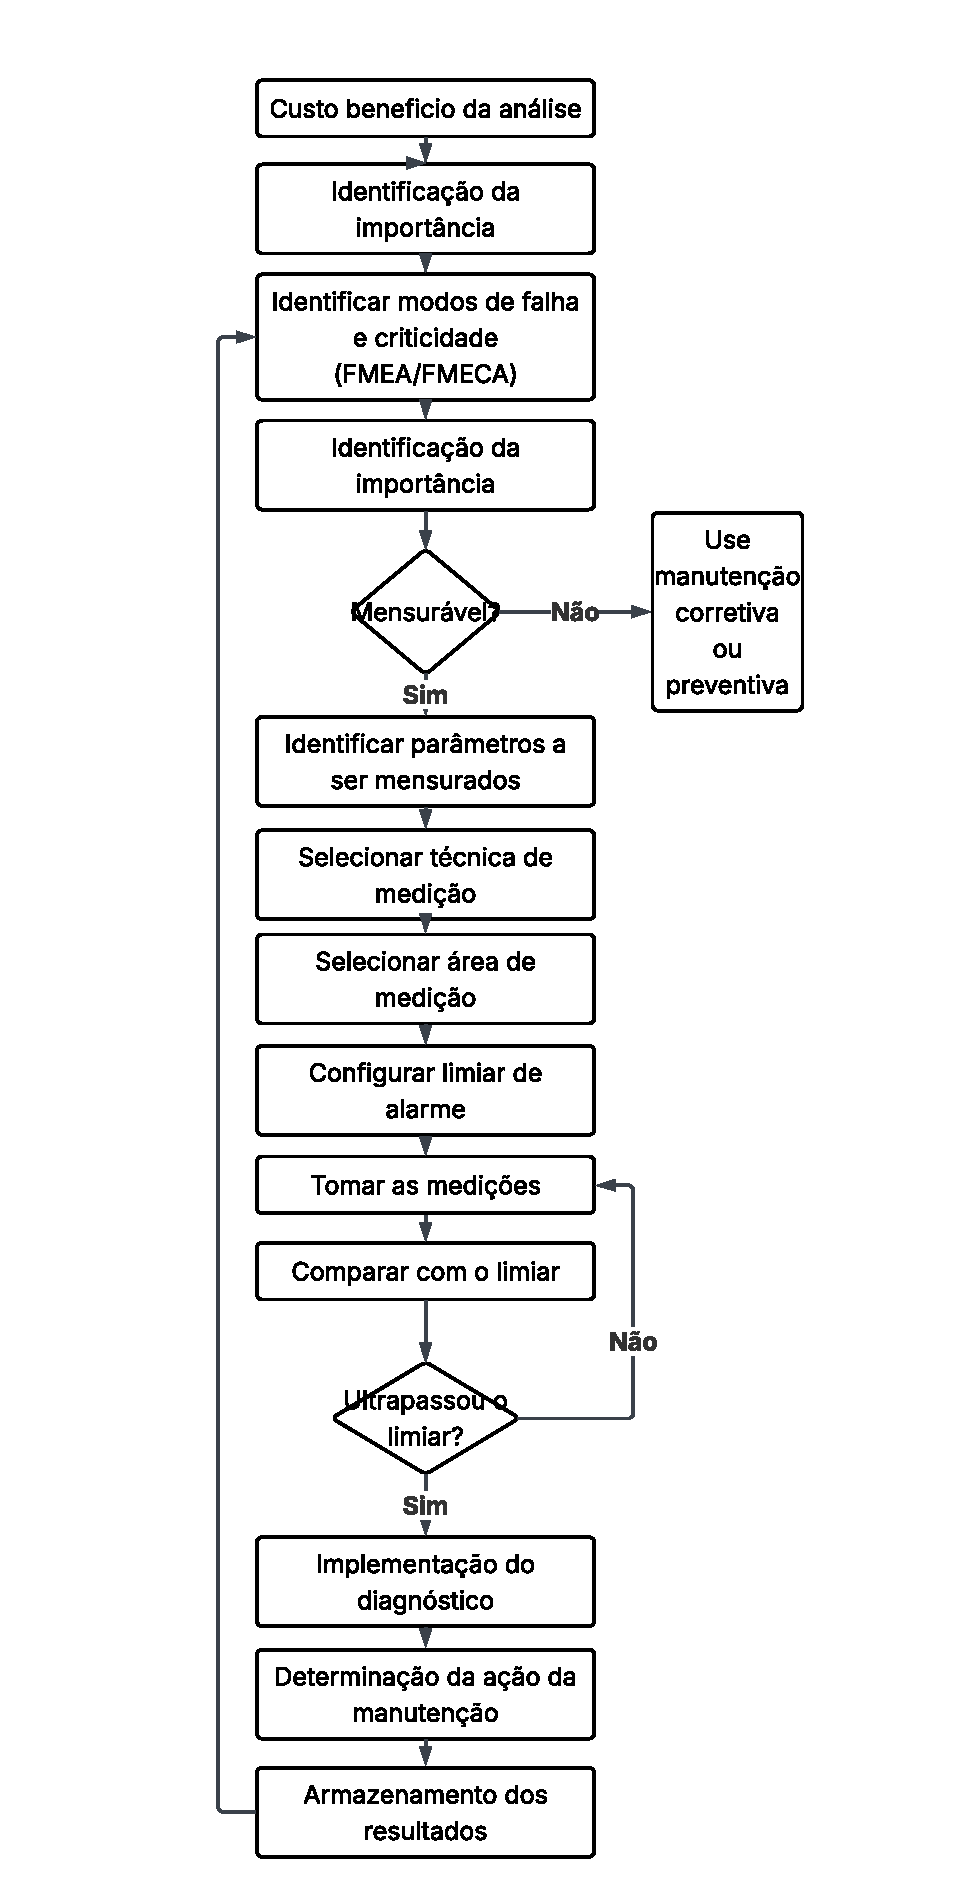
\includegraphics[width=0.8\columnwidth]{Figuras/diagrama.pdf}
    \caption{Procedimento geral para monitoramento de condição e diagnóstico de máquinas, adaptado de \cite{iso17359_2018}.}
    \label{fig:fluxograma_manutencao}
\end{figure}

Entre as diferentes grandezas utilizadas no monitoramento preditivo, a vibração apresenta especial relevância para máquinas rotativas. Falhas mecânicas podem modificar a assinatura vibratória do equipamento, produzindo alterações detectáveis no domínio do tempo e da frequência. A utilização de técnicas de Processamento Digital de Sinais permite extrair características desses sinais e relacioná-las a diferentes condições de operação e modos de falha \cite{randall2011vibration}. Nesse contexto, a análise de vibração constitui a base do sistema de monitoramento desenvolvido neste trabalho, no qual os sinais são adquiridos por um sensor acelerométrico e posteriormente processados para auxiliar no diagnóstico das condições do equipamento.

\subsection{Análise de Vibração e Processamento Digital de Sinais}

A vibração pode ser definida como um movimento oscilatório de um sistema em torno de uma posição de equilíbrio, sendo uma característica inerente ao funcionamento de máquinas e equipamentos rotativos \cite{girdhar2004practical}. No contexto do monitoramento de condição, esse comportamento pode ser mensurado por meio de sensores acelerométricos, permitindo a aquisição das componentes da vibração nos eixos ortogonais $x$, $y$ e $z$.

Cada componente do sinal pode apresentar diferentes amplitudes, frequências e fases e, de forma simplificada, pode ser representada por uma composição de componentes harmônicas. Para uma componente de frequência $f_i$, as acelerações medidas nos três eixos podem ser representadas por

\begin{equation}
x_i(t) = A_i \sin(2\pi f_i t + \phi_i),
\label{equation:x_move}
\end{equation}

\begin{equation}
y_i(t) = B_i \sin(2\pi f_i t + \theta_i),
\label{equation:y_move}
\end{equation}

\begin{equation}
z_i(t) = C_i \sin(2\pi f_i t + \alpha_i),
\label{equation:z_move}
\end{equation}

em que $A_i$, $B_i$ e $C_i$ representam as amplitudes das componentes nos respectivos eixos, $f_i$ corresponde à frequência da componente harmônica e $\phi_i$, $\theta_i$ e $\alpha_i$ representam suas respectivas fases.

A análise desses sinais pode ser realizada tanto no domínio do tempo quanto no domínio da frequência. No domínio do tempo, a representação do sinal permite avaliar a evolução da amplitude da vibração e extrair indicadores estatísticos, como o valor eficaz (\textit{Root Mean Square} -- RMS). Quando expresso em velocidade de vibração (mm/s), esse indicador pode ser utilizado para avaliar a severidade vibratória do equipamento, conforme sua classe de aplicação, estabelecida de acordo com características construtivas e porte da máquina, conforme apresentado no Quadro~\ref{quadro:severidade}. Essa classificação permite relacionar quantitativamente o nível de vibração medido com diferentes condições de operação, auxiliando na avaliação da condição do equipamento. No domínio da frequência, por sua vez, a análise espectral possibilita identificar as componentes de frequência presentes no sinal. Para essa finalidade, emprega-se a Transformada Discreta de Fourier (DFT), cuja implementação computacional eficiente pode ser realizada por meio da Transformada Rápida de Fourier (\textit{Fast Fourier Transform} -- FFT). A representação no domínio da frequência permite, portanto, identificar componentes espectrais associadas ao comportamento dinâmico do equipamento \cite{girdhar2004practical,randall2011vibration}.

\begin{table}[!t]
\centering
\renewcommand{\tablename}{Quadro}
\renewcommand{\arraystretch}{1.3}
\small
\begin{tabular}{|C{1.05cm}|C{1.05cm}|C{1.05cm}|C{1.05cm}|C{1.05cm}|C{1.05cm}|}
\hline
\textbf{$x_{\text{rms}}$ (mm/s)} &
\textbf{$x_{\text{pico}}$ (mm/s)} &
\textbf{Classe I} &
\textbf{Classe II} &
\textbf{Classe III} &
\textbf{Classe IV} \\
\hline

0,28 & 0,50 &
\cellcolor{green!30} Bom &
\cellcolor{green!30} Bom &
\cellcolor{green!30} Bom &
\cellcolor{green!30} Bom \\
\hline

0,45 & 0,76 &
\cellcolor{green!30} Bom &
\cellcolor{green!30} Bom &
\cellcolor{green!30} Bom &
\cellcolor{green!30} Bom \\
\hline

0,71 & 1,01 &
\cellcolor{green!30} Bom &
\cellcolor{green!30} Bom &
\cellcolor{green!30} Bom &
\cellcolor{green!30} Bom \\
\hline

1,12 & 1,52 &
\cellcolor{green!50} Aceitável &
\cellcolor{green!30} Bom &
\cellcolor{green!30} Bom &
\cellcolor{green!30} Bom \\
\hline

1,80 & 2,54 &
\cellcolor{yellow!40} Atenção &
\cellcolor{green!50} Aceitável &
\cellcolor{green!30} Bom &
\cellcolor{green!30} Bom \\
\hline

2,80 & 4,06 &
\cellcolor{yellow!40} Atenção &
\cellcolor{yellow!40} Atenção &
\cellcolor{green!50} Aceitável &
\cellcolor{green!30} Bom \\
\hline

4,50 & 6,35 &
\cellcolor{red!40} Crítico &
\cellcolor{yellow!40} Atenção &
\cellcolor{yellow!40} Atenção &
\cellcolor{green!50} Aceitável \\
\hline

7,10 & 10,16 &
\cellcolor{red!40} Crítico &
\cellcolor{red!40} Crítico &
\cellcolor{yellow!40} Atenção &
\cellcolor{yellow!40} Atenção \\
\hline

11,20 & 15,75 &
\cellcolor{red!40} Crítico &
\cellcolor{red!40} Crítico &
\cellcolor{red!40} Crítico &
\cellcolor{red!40} Crítico \\
\hline

18,00 & 25,40 &
\cellcolor{red!40} Crítico &
\cellcolor{red!40} Crítico &
\cellcolor{red!40} Crítico &
\cellcolor{red!40} Crítico \\
\hline

28,00 & 39,62 &
\cellcolor{red!40} Crítico &
\cellcolor{red!40} Crítico &
\cellcolor{red!40} Crítico &
\cellcolor{red!40} Crítico \\
\hline

45,00 & 63,75 &
\cellcolor{red!40} Crítico &
\cellcolor{red!40} Crítico &
\cellcolor{red!40} Crítico &
\cellcolor{red!40} Crítico \\
\hline

\end{tabular}

\vspace{0.1cm}
\caption{Quadro de Severidade de Velocidade de Vibração}

\label{quadro:severidade}

{\footnotesize Fonte: Adaptado de \cite{santos2023analise} e \cite{iso10816}.}

\end{table}

\renewcommand{\tablename}{Table}
No Quadro \ref{quadro:diagnostico_defeitos} é apresentado a correlação entre falhas comuns e suas manifestações espectrais. Para o processamento da FFT, o sinal deve ter comprimento finito, o que exige o uso de funções de janelamento. No escopo deste trabalho, utiliza-se a janela de Hamming \cite{girdhar2004practical}, cuja resposta em frequência reduz o vazamento espectral (\textit{spectral leakage}) para as bandas vizinhas. Vale ressaltar que janelas mais curtas aumentam a resolução temporal, porém sacrificam a resolução em frequência.
\begin{table*}[!t] % O asterisco faz o quadro ocupar a largura das duas colunas
\centering

% Truque para renomear temporariamente "Table" para "Quadro" no IEEE
\renewcommand{\tablename}{Quadro}

% Garante que as colunas tipo X centralizem verticalmente (m)
\renewcommand{\tabularxcolumn}[1]{m{#1}}

\begin{tabularx}{\textwidth}{|>{\centering\arraybackslash}X|>{\centering\arraybackslash}X|>{\centering\arraybackslash}X|>{\centering\arraybackslash}X|}
\hline
\rowcolor[HTML]{EFEFEF} 
\textbf{Defeito Mecânico} & \textbf{Assinatura no Espectro} & \textbf{Característica no Tempo} & \textbf{Direção Predominante} \\ \hline
Desbalanceamento & Pico alto e único em 1x RPM (frequência de rotação). & Senoide limpa e repetitiva. & Radial (Horizontal ou Vertical). \\ \hline
Desalinhamento & Picos em 1x, 2x (muito comum) e às vezes 3x RPM. & Onda levemente "achatada" ou com dupla crista. & Axial (ao longo do eixo). \\ \hline
Folga Mecânica & Muitas harmônicas (1x, 2x, 3x... 10x) e às vezes sub-harmônicas (0.5x). & Impactos aleatórios ou batimentos irregulares. & Radial (geralmente Vertical). \\ \hline
Falha de Rolamento & Picos em frequências não-síncronas (ex: 7,42x RPM) e bandas laterais. & Pulsos de choque agudos e repetitivos (impactos). & Radial e Axial. \\ \hline
Cavitação (Bombas) & Ruído de fundo elevado (piso do gráfico sobe) em altas frequências. & Ruído aleatório. & Todas as direções. \\ \hline
\end{tabularx}

\vspace{4pt}
% Substitui o \legend do ABNTeX2

\caption{Diagnóstico de defeitos mecânicos e suas assinaturas vibratórias.}
\label{quadro:diagnostico_defeitos}
\vspace{0.1cm}
{\footnotesize Fonte: Adaptado de \cite{randall2011vibration}.}

% Retorna o nome padrão caso existam outras tabelas no artigo
\renewcommand{\tablename}{Table} 
\end{table*}
Apesar de sua ampla aplicação na análise de vibrações, a transformada de Fourier apresenta uma limitação associada à resolução temporal e espectral. Para uma determinada janela de aquisição, a resolução em frequência depende da duração do sinal analisado, de modo que a utilização de janelas mais longas proporciona maior resolução espectral, mas reduz a capacidade de localizar temporalmente variações rápidas do sinal. Dessa forma, a representação espectral obtida pela DFT caracteriza o conteúdo em frequência da janela analisada, mas não fornece diretamente a localização temporal dos eventos que originaram cada componente espectral \cite{oppenheim2010discrete}. Essa característica pode limitar a análise de fenômenos transitórios ou de curta duração, especialmente quando alterações relevantes ocorrem em intervalos reduzidos.

Como alternativa para a análise de sinais não estacionários, a Transformada Wavelet fornece uma representação simultaneamente relacionada à escala e à localização temporal do sinal. Essa transformação utiliza uma função denominada \textit{wavelet-mãe}, a partir da qual são obtidas funções com diferentes escalas e deslocamentos. A variação da escala permite analisar diferentes características do sinal, enquanto o deslocamento possibilita localizar essas características ao longo do tempo \cite{randall2011vibration}.

A Transformada Wavelet Contínua (CWT) pode ser expressa por (\ref{equation:wavelet}):

\begin{equation}
W(a,b) =
\frac{1}{\sqrt{a}}
\int_{-\infty}^{+\infty}
x(t)\psi^{*}
\left(
\frac{t-b}{a}
\right)dt,
\label{equation:wavelet}
\end{equation}

em que $x(t)$ representa o sinal analisado, $\psi(t)$ corresponde à wavelet-mãe, $a$ representa o fator de escala, $b$ o parâmetro de deslocamento temporal e $\psi^{*}$ o complexo conjugado da função wavelet.

Neste trabalho, emprega-se a wavelet de \textit{Morlet}, definida por (\ref{equation:morlet}):

\begin{equation}
\psi(t) =
\frac{\sigma}{\sqrt{\pi}}
e^{-\sigma^2 t^2}
e^{j2\pi f_0t},
\label{equation:morlet}
\end{equation}

Por apresentar características adequadas à análise de sinais oscilatórios e transitórios. A utilização de diferentes escalas permite analisar características do sinal associadas a diferentes faixas de frequência, enquanto o parâmetro de deslocamento possibilita identificar sua ocorrência ao longo do tempo. Essa característica torna a análise wavelet particularmente adequada para sinais de vibração que apresentam componentes transitórias ou variações rápidas, como impactos mecânicos e eventos associados ao desenvolvimento de determinadas falhas em componentes rotativos \cite{randall2011vibration}.

Outra técnica complementar empregada na análise de vibrações é a Transformada de Hilbert, particularmente útil na análise de sinais modulados e na extração da envoltória. Essa abordagem pode ser utilizada para evidenciar componentes periódicas associadas a eventos de impacto, sendo especialmente relevante na identificação de falhas incipientes em rolamentos \cite{randall2011vibration}. A Transformada de Hilbert de um sinal $x(t)$ é definida por (\ref{equation:hilbert}).

\begin{equation}
\tilde{x}(t) =
\frac{1}{\pi}
\int_{-\infty}^{+\infty}
\frac{x(\tau)}{t-\tau}\tau
\label{equation:hilbert}
\end{equation}

em que $\tilde{x}(t)$ representa a Transformada de Hilbert de $x(t)$. A partir dessa transformação, pode-se construir o sinal analítico, conforme apresentado na Equação (\ref{equation:analitico}).

\begin{equation}
z(t) = x(t) + j\tilde{x}(t)
\label{equation:analitico}
\end{equation}

cuja magnitude fornece a envoltória do sinal, apresentado por (\ref{equation:module}).

\begin{equation}
x_e(t) = |z(t)|
= \sqrt{x^2(t)+\tilde{x}^2(t)}.
\label{equation:module}
\end{equation}

A análise da envoltória permite evidenciar modulações associadas a impactos periódicos, possibilitando a identificação de componentes relacionadas às frequências características de falhas em elementos rotativos. Dessa forma, a Transformada de Hilbert constitui uma ferramenta complementar à análise espectral convencional.


% No contexto deste artigo, a FFT é empregada na caracterização do conteudo espectral. Graças à FFT é possível, através da função de janelamento adotada, analisar a influência de cada  componente harmônica na construção do sinal de vibração, porém ao aumentar o janelamento, escala em frequência, ocorre uma perda de resolução no tempo e vice versa. Para contornar esse problema, é utilizado a transformada de \textit{wavelet}, que utili
No contexto deste artigo, a FFT é empregada para a caracterização do conteúdo espectral dos sinais de vibração, contribuindo para o isolamento e a identificação de componentes e frequências predominantes associadas a falhas específicas, como o desbalanceamento. A Transformada Wavelet é utilizada para a análise de fenômenos não estacionários, contribuindo com uma representação simultânea de alta resolução no tempo e na frequência, o que permitiu localizar e evidenciar eventos transitórios de curta duração, como impactos mecânicos rápidos. Por sua vez, a Transformada de Hilbert é aplicada para a análise da envoltória, contribuindo para a demodulação do sinal e a revelação de falhas prematuras e incipientes em rolamentos (frequências de defeito como BPFO e BPFI) que atuariam em altas frequências e seriam imperceptíveis na análise espectral convencional devido aos baixos níveis de amplitude. A utilização conjunta dessas técnicas permite explorar diferentes características dos sinais adquiridos e fornece informações complementares para o diagnóstico da condição do equipamento.

\section{Metodologia do Sistema}

O presente trabalho caracteriza-se como uma pesquisa aplicada, tendo como objetivo o desenvolvimento de uma solução para o monitoramento e a análise de vibrações mecânicas. O sistema foi desenvolvido com foco em aplicações de manutenção preditiva, buscando fornecer dados que auxiliem na avaliação da condição de equipamentos industriais e na identificação de alterações em seu comportamento vibratório.

\subsection{Hardware}

O desenvolvimento do sistema foi realizado de forma incremental, contemplando inicialmente a seleção dos componentes e o desenvolvimento do dispositivo de aquisição. Para a medição das vibrações, foi empregado o acelerômetro ADXL345, selecionado em função de sua capacidade de aquisição em alta taxa de amostragem e de sua resolução, além da relação entre custo e desempenho para a aplicação proposta.

Como unidade de processamento, foi utilizado o microcontrolador XIAO ESP32-C6, da Seeed Studio, escolhido em função de sua capacidade de processamento, recursos de comunicação e baixo consumo de energia. A alimentação do dispositivo foi realizada por meio de uma bateria de íons de lítio, modelo 602535, com capacidade de 600~mAh, associada a um módulo TP4056 para gerenciamento do carregamento. O módulo também permite a alimentação do sistema durante o processo de carregamento, possibilitando a operação em \textit{bypass}.

Para a integração dos componentes, foi desenvolvida uma placa de circuito impresso destinada à conexão entre o microcontrolador, o acelerômetro e os demais elementos do sistema. A utilização da placa permitiu reduzir as dimensões do conjunto e organizar as conexões elétricas, resultando no dispositivo apresentado nas Figuras~\ref{fig:imagem_a} e~\ref{fig:imagem_b}.

\begin{figure}[!t]
    \centering
    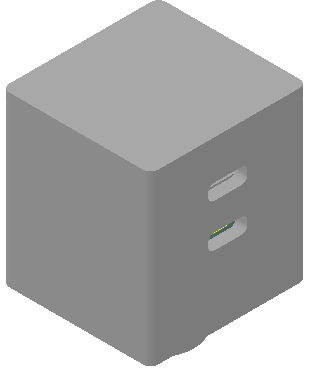
\includegraphics[width=0.5\columnwidth]{Figuras/prot_01.png}
    \caption{Vista em perspectiva isométrica do dispositivo desenvolvido.}
    \label{fig:imagem_a}
    
    {\footnotesize Fonte: Elaborado pelo autor.}
\end{figure}

\begin{figure}[!t]
    \centering
    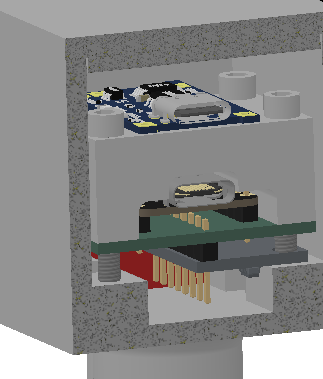
\includegraphics[width=0.5\columnwidth]{Figuras/proto_03.png}
    \caption{Vista em corte do dispositivo desenvolvido.}
    \label{fig:imagem_b}
    
    {\footnotesize Fonte: Elaborado pelo autor.}
\end{figure}

O custo aproximado dos componentes utilizados no protótipo é apresentado na Tabela~\ref{tab:custos_componentes}, evidenciando o baixo custo de implementação do sistema.

\renewcommand{\tablename}{Quadro}
\begin{table}[!t]
    \centering
    \caption{Estimativa de custos dos componentes do protótipo.}
    \label{tab:custos_componentes}
    \vspace{0.2cm}
    
    \begin{tabular}{lc}
        \toprule
        \textbf{Componente} & \textbf{Custo aproximado} \\
        \midrule
        XIAO ESP32-C6 & R\$ 50,00 \\
        ADXL345 & R\$ 20,00 \\
        Case 3D & -- \\
        TP4056 & R\$ 10,00 \\
        Bateria 602535 & R\$ 40,00 \\
        Placa de circuito impresso & -- \\
        \bottomrule
    \end{tabular}
    
    \vspace{0.2cm}
    {\footnotesize Fonte: Elaborado pelo autor.}
\end{table}
    
\renewcommand{\tablename}{Table}
\subsection{Software}
Para o desenvolvimento do firmware do microcontrolador XIAO ESP32-C6, foi utilizada a linguagem C++, empregando o ambiente \textit{PlatformIO} como extensão do \textit{Visual Studio Code}. A utilização dessa ferramenta possibilitou o gerenciamento das dependências do projeto, a configuração da plataforma de desenvolvimento e a organização do código destinado à aquisição e ao processamento inicial dos sinais de vibração.

A interface gráfica e o processamento dos dados foram desenvolvidos em \textit{Python}, utilizando o \textit{framework PySide6} para a construção da interface. A biblioteca \textit{NumPy} foi empregada para a manipulação e o processamento dos dados numéricos, enquanto a biblioteca \textit{SciPy} foi utilizada na aplicação de métodos de processamento digital de sinais, incluindo as transformadas de Fourier e de Hilbert.

Para o armazenamento e o gerenciamento dos dados em nuvem, foi utilizada a biblioteca \textit{firebase-admin}, responsável pela integração da aplicação com o banco de dados \textit{Firebase}. Essa estrutura permitiu o armazenamento de informações relacionadas aos equipamentos monitorados, usuários e alarmes.

Para o desenvolvimento e a organização do software, foram utilizados os ambientes \textit{Visual Studio Code} e \textit{PyCharm}. Adicionalmente, o \textit{Qt Designer} foi empregado na concepção da interface gráfica, permitindo a elaboração visual dos elementos da aplicação e reduzindo a necessidade de implementação manual dos componentes da interface por meio do \textit{PySide6}.

\section{Desenvolvimento do Sistema Proposto}

\subsection{Arquitetura do Sistema}

O sistema proposto foi desenvolvido para realizar a aquisição, transmissão e análise de sinais de vibração, utilizando o acelerômetro \textit{ADXL345} para a aquisição dos dados de aceleração e o microcontrolador XIAO ESP32-C3 para o processamento inicial e o gerenciamento da comunicação. A arquitetura desenvolvida permite três modos distintos de operação, configuráveis por meio da interface supervisória: \textit{online}, \textit{offline} e \textit{serial}.

No modo \textit{online}, também denominado monitoramento contínuo, o dispositivo permanece conectado à Internet por meio de uma rede \textit{Wi-Fi} e realiza a transmissão dos dados utilizando o protocolo \textit{WebSocket}. A utilização desse protocolo permite o estabelecimento de uma comunicação bidirecional entre o dispositivo e o computador, mantendo a conexão disponível para o envio e o recebimento de dados. Para a operação nesse modo, o usuário deve configurar o endereço IP do computador, as credenciais da rede \textit{Wi-Fi} e selecionar o modo correspondente na interface supervisória antes do início da aquisição. A principal limitação dessa configuração está relacionada ao consumo de energia, que pode atingir aproximadamente 220~mA durante a transmissão, tornando necessária, em aplicações prolongadas, a utilização de uma fonte de alimentação externa, em função da capacidade limitada da bateria de 600~mAh.

O modo \textit{offline} foi desenvolvido com o objetivo de reduzir o consumo energético do dispositivo. Nessa configuração, o sensor realiza aquisições periódicas previamente programadas e, caso seja identificado um valor de velocidade RMS ou pico de vibração superior ao limiar estabelecido na interface supervisória, os dados da aquisição são armazenados em formato binário (arquivo com extensão .bin) e, posteriormente, disponibilizados por meio do \textit{Google Drive}. A utilização dessa plataforma permite a sincronização dos arquivos com o computador do operador, possibilitando que os dados adquiridos sejam acessados e processados pela interface gráfica. Dessa forma, o sistema permite a realização de análises semelhantes às disponíveis no monitoramento contínuo, mesmo sem a necessidade de manter o dispositivo permanentemente conectado à rede.

O modo \textit{serial} foi desenvolvido para aplicações nas quais se deseja reduzir a latência da comunicação e utilizar uma fonte de alimentação estável por meio da interface USB. Nessa configuração, a alimentação do dispositivo é realizada diretamente pelo barramento USB, eliminando a dependência da bateria durante a operação. As verificações de alarme são iniciadas manualmente pelo operador por meio do comando ``MODO SERIAL'' disponibilizado na interface supervisória.

Além dos modos de aquisição, o sistema possui uma arquitetura destinada ao monitoramento e à análise dos sinais adquiridos. Após o início de uma aquisição, a interface supervisória recebe as amostras e apresenta os sinais nos domínios do tempo e da frequência. A partir dos dados de aceleração obtidos, é calculada a velocidade por meio das seguintes etapas: remoção do \textit{offset}, aplicação de um filtro digital, integração numérica, remoção da tendência linear e, por fim, aplicação de um segundo filtro digital. Em seguida, a partir do sinal de velocidade, são calculados o valor RMS e o valor de pico da vibração. Esses parâmetros são comparados com os limiares de alarme definidos pelo usuário, os quais são independentes dos limites de severidade estabelecidos pela norma ISO 10816, conforme apresentado no Quadro~\ref{quadro:niveis_severidade}.

Quando os valores de RMS ou de pico ultrapassam os respectivos limiares configurados, o sistema verifica a existência de alarmes previamente registrados durante o ciclo de monitoramento vigente. Na ausência de um alarme anterior, são executados os algoritmos de processamento digital de sinais (PDS) empregados para a identificação das características associadas ao aumento da energia vibratória. A partir dos resultados obtidos, é realizada a estimativa da possível condição de falha, sendo posteriormente encaminhado um e-mail contendo o diagnóstico provável.

Caso os valores de RMS e de pico permaneçam abaixo dos limiares estabelecidos, ou já exista um alarme registrado no ciclo de monitoramento, o sistema mantém o monitoramento e a atualização das representações gráficas, sem executar novamente o processo de diagnóstico.

A definição dos limiares personalizados de RMS e de pico é de responsabilidade do usuário administrador do sistema. Como referência para essa configuração, o sistema disponibiliza os limites de severidade estabelecidos pela norma ISO 10816, considerando os diferentes níveis de severidade e as classes de equipamentos, conforme apresentado no Quadro~\ref{quadro:niveis_severidade}. Dessa forma, o operador pode estabelecer limiares específicos dentro das faixas de severidade apresentadas pela norma. Por exemplo, caso seja desejado que o alarme seja acionado somente quando o nível de vibração atingir a condição crítica, o limiar pode ser configurado próximo ao limite correspondente a essa condição.

\subsection{\textit{Software} Supervisório}

Foi desenvolvido um \textit{software} supervisório destinado à visualização e à análise dos sinais de vibração em tempo real, bem como ao gerenciamento dos equipamentos monitorados. Cada equipamento possui um histórico próprio, no qual são registrados os alarmes emitidos, os diagnósticos realizados e os respectivos planos de manutenção.

A tela inicial do supervisório é apresentada na Figura~\ref{fig:supervisorio}, na qual são destacadas as principais funcionalidades disponíveis:

\begin{enumerate}
    \item status da conexão \textit{Wi-Fi} do XIAO ESP32-C3;
    \item status da conexão \textit{WebSocket} com o dispositivo;
    \item seleção do equipamento a ser monitorado;
    \item processamento de arquivos adquiridos durante o modo \textit{offline};
    \item indicação do status da aquisição em tempo real;
    \item seleção do tipo de análise;
    \item configurações dos parâmetros de análise;
    \item definição dos limiares de RMS e de pico para a emissão de alarmes;
    \item início da aquisição pelo supervisório;
    \item interrupção da aquisição pelo supervisório;
    \item início da aquisição por comunicação serial;
    \item visualização dos sinais em tempo real;
    \item apresentação dos valores calculados em tempo real.
\end{enumerate}

Além da tela inicial, o \textit{software} dispõe de outras interfaces destinadas à análise e ao gerenciamento das informações obtidas durante o monitoramento. A tela de análise permite a visualização gráfica dos resultados das técnicas de processamento digital de sinais empregadas no sistema, incluindo a FFT, a Transformada Wavelet, a Transformada de Hilbert e a análise cepstral. O sistema também dispõe de interfaces destinadas ao gerenciamento de alarmes, apresentação dos diagnósticos, acompanhamento dos níveis de severidade e gerenciamento dos planos de manutenção dos equipamentos.

\begin{figure}[!t]
    \centering
    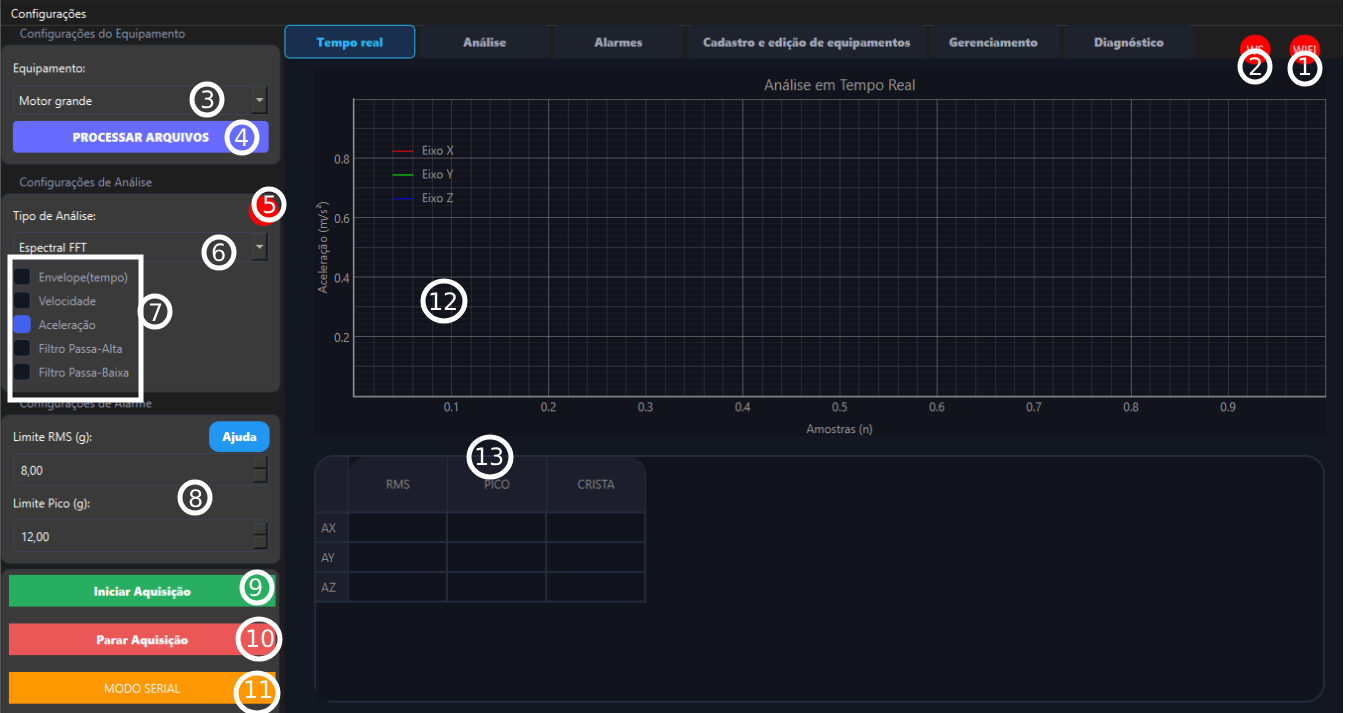
\includegraphics[width=\columnwidth]{Figuras/supervisorioMain.png}
    \caption{Tela inicial do software supervisório.}
    \label{fig:supervisorio}
    
    {\footnotesize Fonte: Elaborado pelo autor.}
\end{figure}


\section{Ensaios com o Protótipo e Sistema Supervisório}

Nesta etapa, o sistema foi submetido a ensaios experimentais com a aplicação das principais ferramentas de processamento digital de sinais abordadas neste trabalho, incluindo a FFT, a análise cepstral, a transformada de Hilbert e a transformada de wavelet. O objetivo desta etapa consiste em avaliar o comportamento do sistema desenvolvido diante de diferentes condições de operação e, posteriormente, verificar sua capacidade de identificar alterações no comportamento vibratório do equipamento.

Os dados nominais do motor utilizado nos ensaios são apresentados na Figura~\ref{fig:dados_motoTeste}. A fixação do protótipo foi realizada por meio de uma fita dupla face posicionada na região central do MIT (Motor de Indução Trifásico), conforme apresentado na Figura~\ref{fig:mit_fix}. O motor foi acionado por meio de um inversor de frequência, modelo CFP, da fabricante ProVolt, configurado para operar a 30 Hz. Essa frequência foi adotada com o objetivo de evitar níveis excessivos de vibração durante os ensaios com carga desbalanceada.

A metodologia experimental consistiu na análise do MIT em três condições distintas: operação sem perturbações externas, operação com desbalanceamento induzido e operação com impactos mecânicos simulados.

\begin{figure}[!t]
    \centering
    \caption{Dados nominais do motor de teste.}
    \label{fig:dados_motoTeste}
    \vspace{0.2cm}
    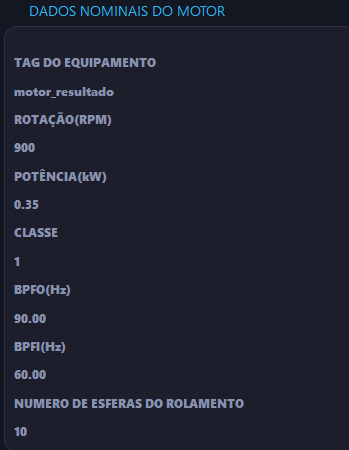
\includegraphics[width=0.5\columnwidth]{Figuras/motoTeste.png}
    \vspace{0.1cm}

    {\footnotesize Fonte: Elaborado pelo autor.}
\end{figure}

\begin{figure}[!t]
    \centering
    \caption{Fixação do protótipo no motor.}
    \label{fig:mit_fix}
    \vspace{0.2cm}
    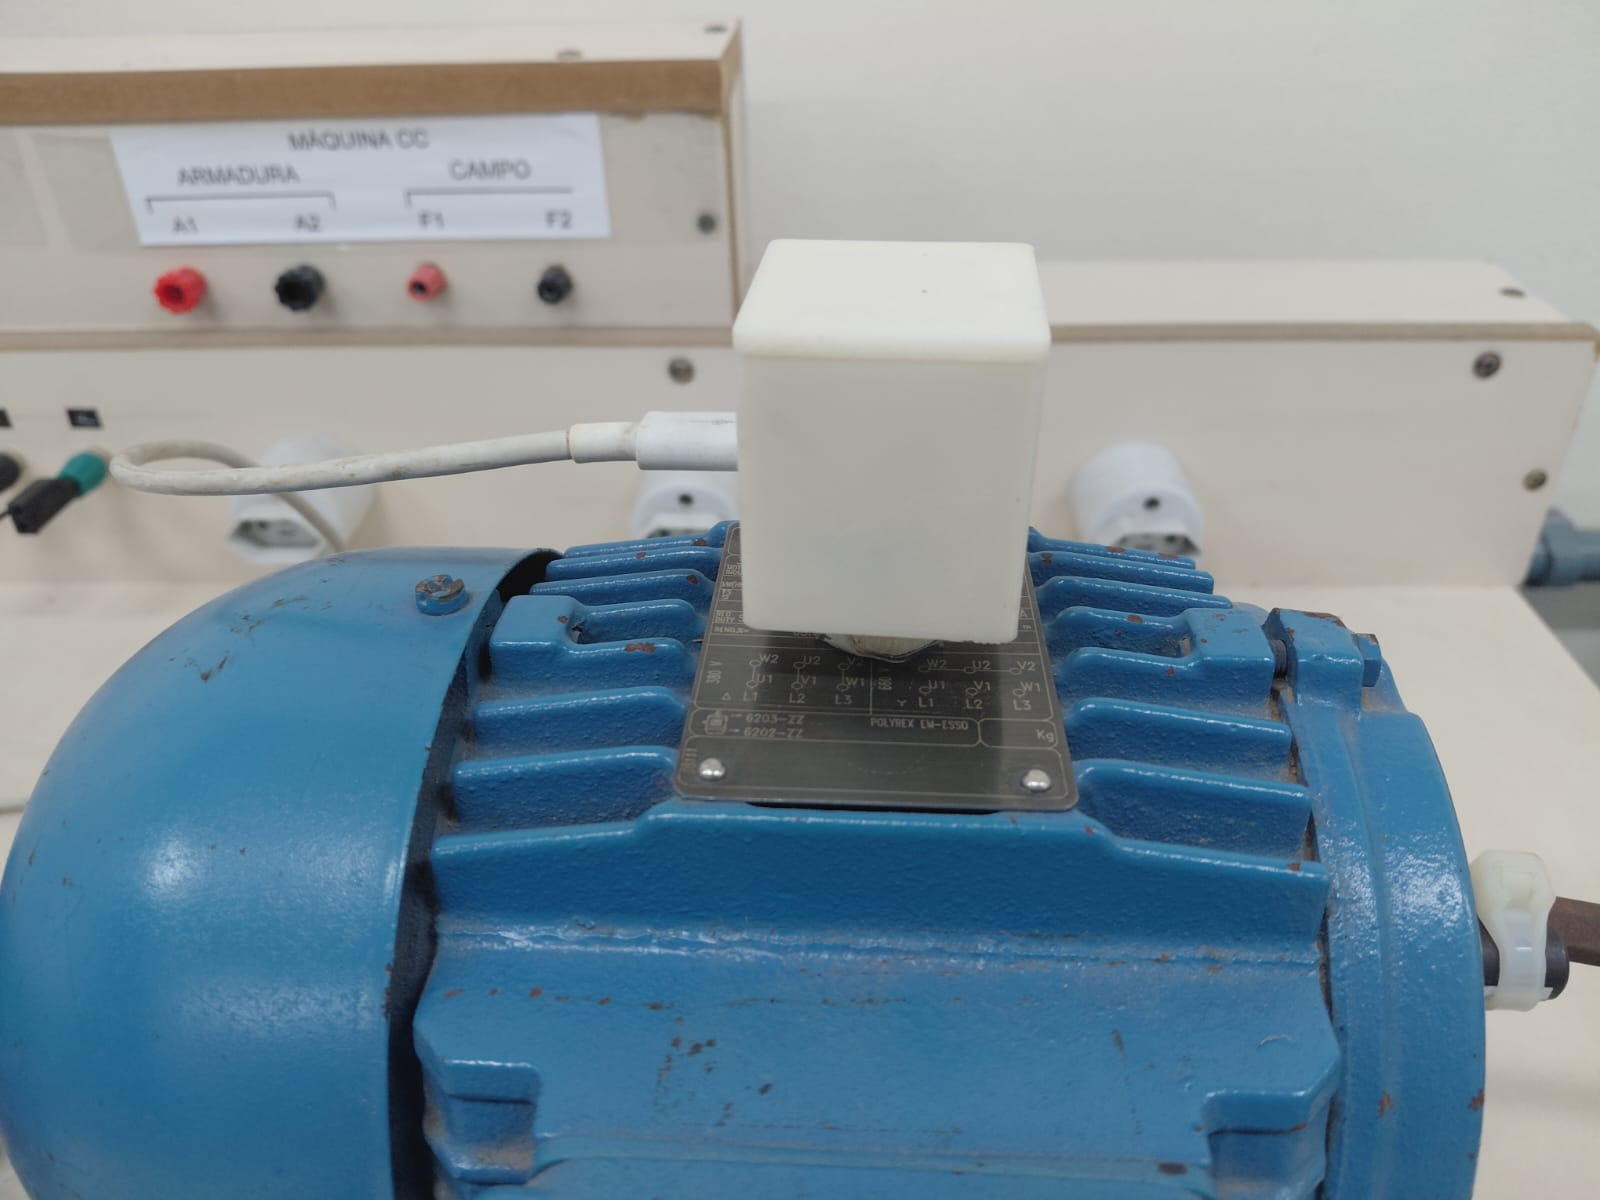
\includegraphics[width=0.95\columnwidth]{Figuras/sensor_fix.jpg}
    \vspace{0.1cm}
    {\footnotesize Fonte: Elaborado pelo autor.}
\end{figure}


\subsection{Análise do MIT sem perturbação}

Inicialmente, foi realizada a análise do MIT em uma condição de operação sem perturbações externas, com o objetivo de estabelecer uma referência para o comportamento vibratório do equipamento. Nessa etapa, foram analisados os sinais de velocidade e aceleração no domínio do tempo, conforme apresentado nas Figuras~\ref{fig:normal_velocidade_30} e~\ref{fig:normal_aceleracao_30}, respectivamente.

Para a faixa de baixa frequência associada à rotação do motor, a análise da velocidade apresenta maior relevância, uma vez que essa grandeza permite avaliar diretamente os níveis globais de vibração por meio dos valores RMS e de pico.

\begin{figure}[!t]
    \centering
    \caption{MIT sem perturbação: sinal de velocidade.}
    \label{fig:normal_velocidade_30}
    \vspace{0.2cm}
    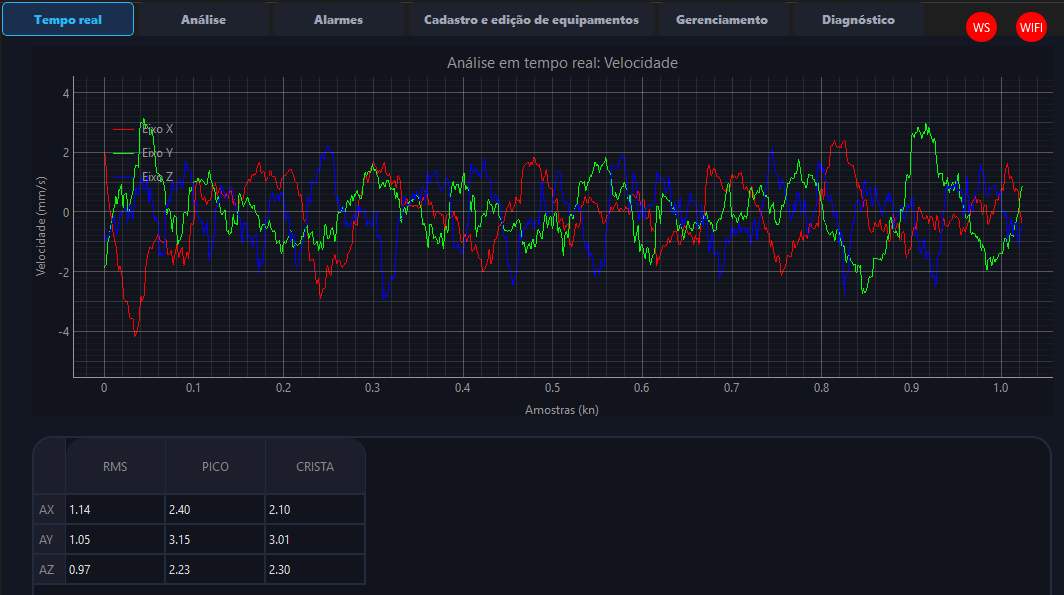
\includegraphics[width=0.95\columnwidth]{Figuras/normal_velocidade_30.png}
    \vspace{0.1cm}
    {\footnotesize Fonte: Elaborado pelo autor.}
\end{figure}

\begin{figure}[!t]
    \centering
    \caption{MIT sem perturbação: sinal de aceleração.}
    \label{fig:normal_aceleracao_30}
    \vspace{0.2cm}
    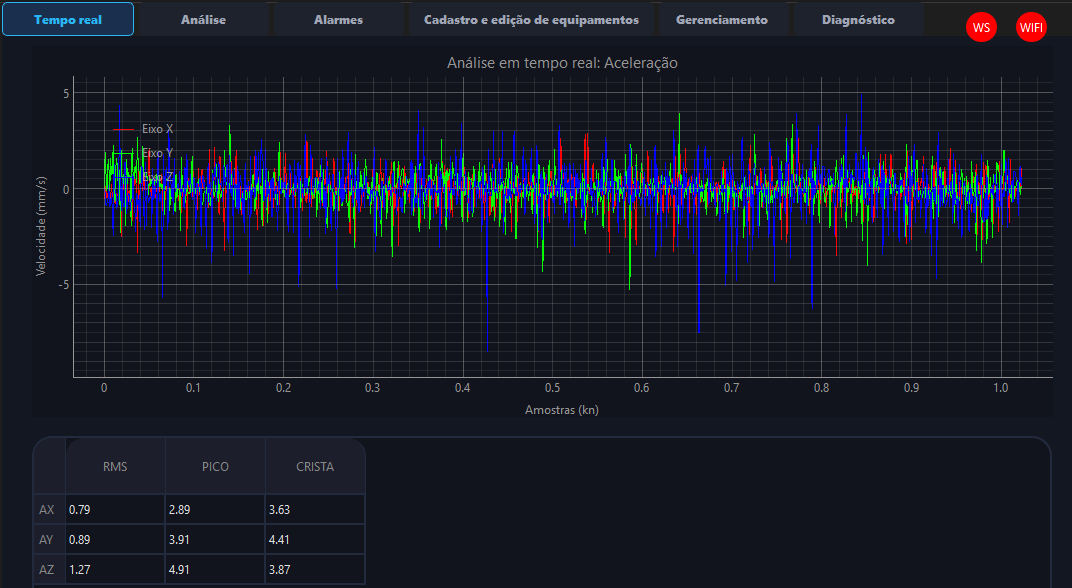
\includegraphics[width=0.95\columnwidth]{Figuras/normal_aceleracao_30.png}
    \vspace{0.1cm}
    {\footnotesize Fonte: Elaborado pelo autor.}
\end{figure}

Na sequência, foi realizada a análise espectral do sinal de velocidade por meio da FFT. O espectro obtido apresentou diversas componentes harmônicas distribuídas aproximadamente entre 0 Hz e 180 Hz, conforme apresentado na Figura~\ref{fig:FFT_velocidade}.

\begin{figure}[!t]
    \centering
    \caption{MIT sem perturbação: FFT do sinal de velocidade.}
    \label{fig:FFT_velocidade}
    \vspace{0.2cm}
    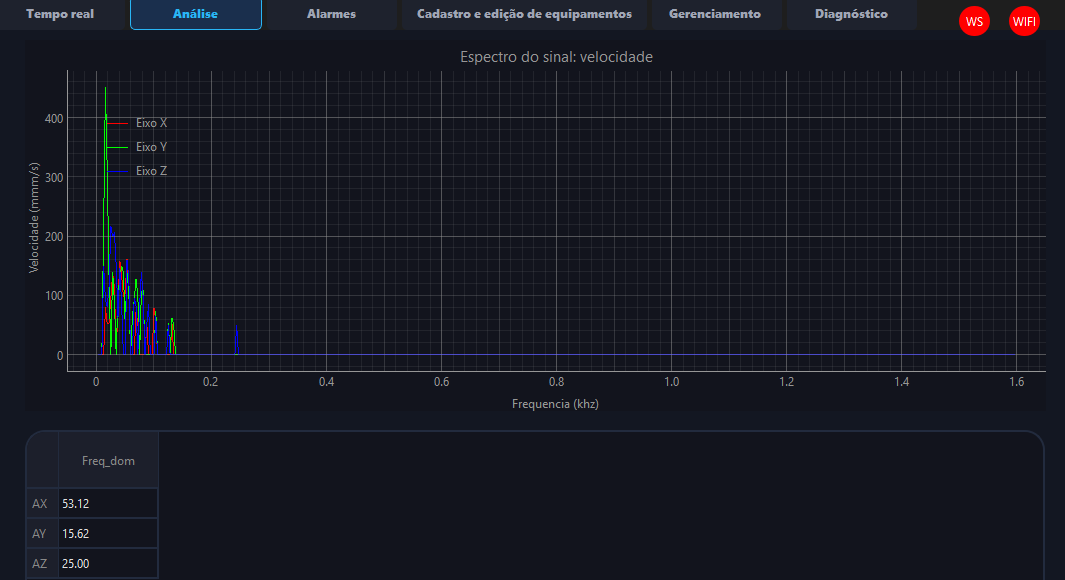
\includegraphics[width=0.95\columnwidth]{Figuras/normal_velocidade_fft_30.png}
    \vspace{0.1cm}
    {\footnotesize Fonte: Elaborado pelo autor.}
\end{figure}

Adicionalmente, a FFT foi aplicada ao sinal de aceleração com o objetivo de avaliar componentes em frequências mais elevadas. Nessa análise, observou-se a presença de múltiplas componentes espectrais distribuídas ao longo da faixa de frequência analisada, conforme apresentado na Figura~\ref{fig:FFT_aceleracao}.

\begin{figure}[!t]
    \centering
    \caption{MIT sem perturbação: FFT do sinal de aceleração.}
    \label{fig:FFT_aceleracao}
    \vspace{0.2cm}
    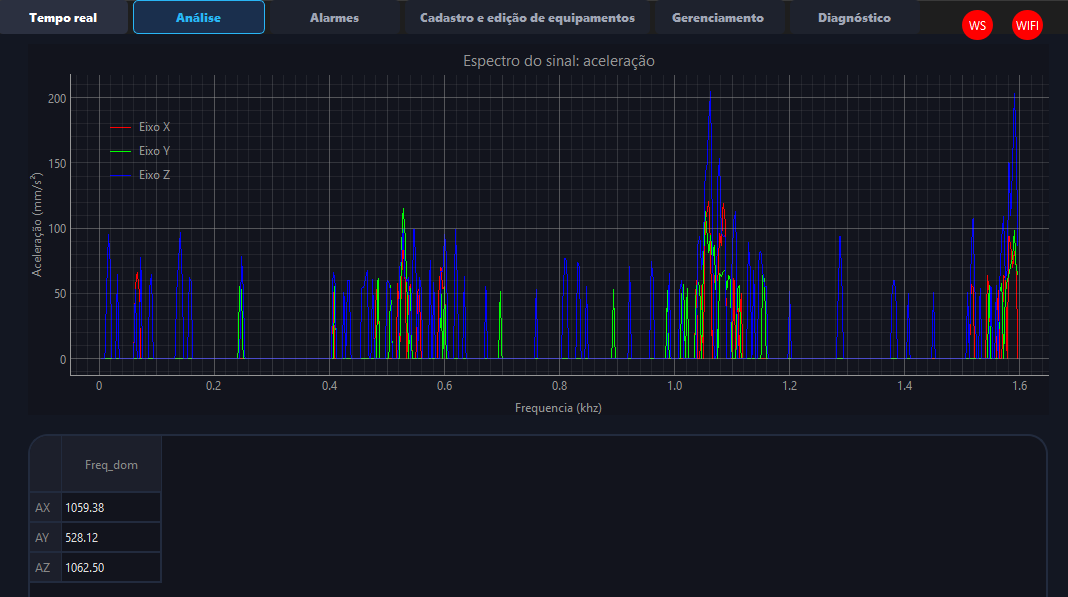
\includegraphics[width=0.95\columnwidth]{Figuras/normal_aceleraca_fft_30.png}
    \vspace{0.1cm}
    {\footnotesize Fonte: Elaborado pelo autor.}
\end{figure}

Em seguida, foi realizada a análise do sinal envelopado, obtido a partir da aplicação da transformada de Hilbert ao sinal de vibração previamente filtrado. Essa abordagem permite investigar componentes de modulação associadas a eventos de impacto e, consequentemente, auxiliar na identificação de características relacionadas a falhas em elementos de rolamentos.

No ensaio realizado, foi utilizado um filtro passa-altas com frequência de corte de 600 Hz. A análise espectral do sinal envelopado apresentou componentes associadas às frequências características de falhas em rolamentos, incluindo componentes relacionadas à BPFO(\textit{Ball Pass Frequency Outer}, frequência de passagem na pista externa) e à BPFI(\textit{Ball Pass Frequency Inner}, frequência de passagem da pista interna), conforme apresentado na Figura~\ref{fig:FFT_hilbert}. Entretanto, essas componentes apresentaram amplitudes relativamente baixas, de modo que não foram suficientes para o acionamento do diagnóstico automático pelo software.

\begin{figure}[!t]
    \centering
    \caption{MIT sem perturbação: FFT do sinal envelopado.}
    \label{fig:FFT_hilbert}
    \vspace{0.2cm}
    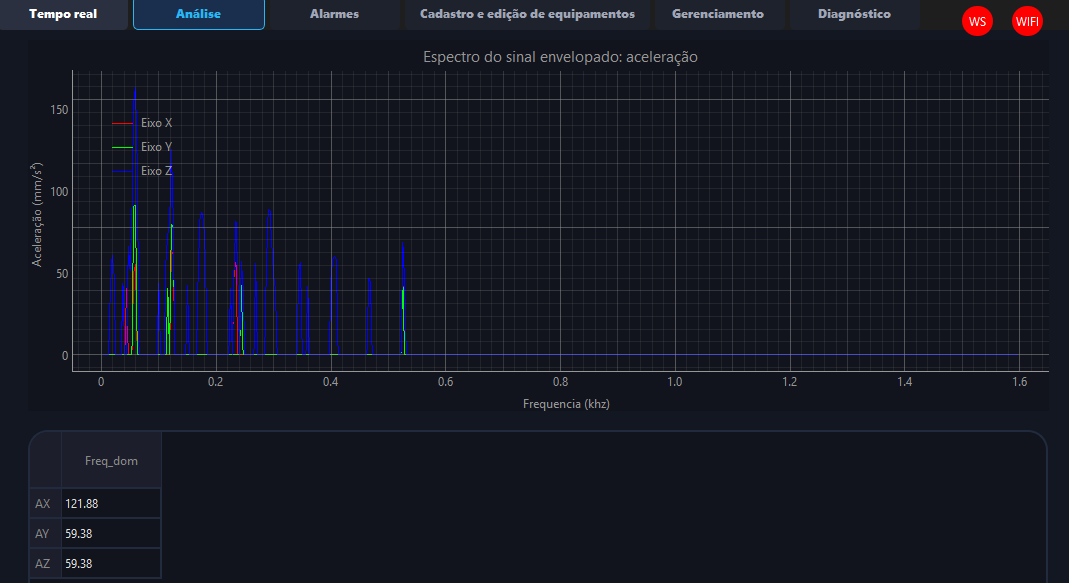
\includegraphics[width=0.95\columnwidth]{Figuras/normal_hilbert_fft_30.png}
    \vspace{0.1cm}
    {\footnotesize Fonte: Elaborado pelo autor.}
\end{figure}

Por fim, foi aplicada a transformada de wavelet ao sinal de aceleração, com o objetivo de avaliar a distribuição das componentes do sinal no domínio tempo-frequência. Essa abordagem permite observar simultaneamente a ocorrência de determinadas componentes espectrais e sua localização temporal, sendo particularmente útil na identificação de eventos transitórios e impactos mecânicos.

Na condição de operação sem perturbações, a análise por wavelet apresentou o comportamento do sinal ao longo do intervalo de aquisição, permitindo estabelecer uma referência para comparação com os ensaios realizados posteriormente. O resultado obtido é apresentado na Figura~\ref{fig:normal_wavelet}.

\begin{figure}[!t]
    \centering
    \caption{MIT sem perturbação: transformada de wavelet.}
    \label{fig:normal_wavelet}
    \vspace{0.2cm}
    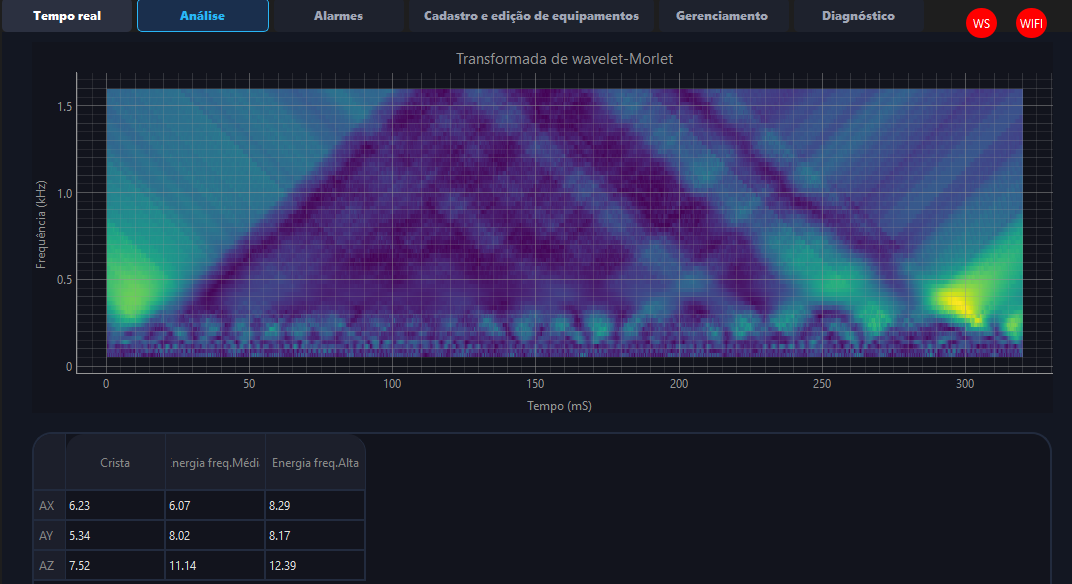
\includegraphics[width=0.95\columnwidth]{Figuras/normal_wavelet_aceleracao_30.png}
    \vspace{0.1cm}
    {\footnotesize Fonte: Elaborado pelo autor.}
\end{figure}


\subsection{Análise do MIT com perturbação: desbalanceamento}

Após a conclusão das análises do motor em condições normais de operação, foi introduzida uma perturbação mecânica no eixo do motor, com o objetivo de provocar uma condição de desbalanceamento. A partir dessa condição, foram repetidas as análises realizadas anteriormente, permitindo comparar o comportamento vibratório do equipamento antes e após a introdução da perturbação.

Para induzir o desbalanceamento, uma chave Allen foi fixada ao eixo do motor por meio de uma abraçadeira plástica, conforme apresentado na Figura~\ref{fig:perturbacaoDesbalanceamento}.

\begin{figure}[!ht]
    \centering
    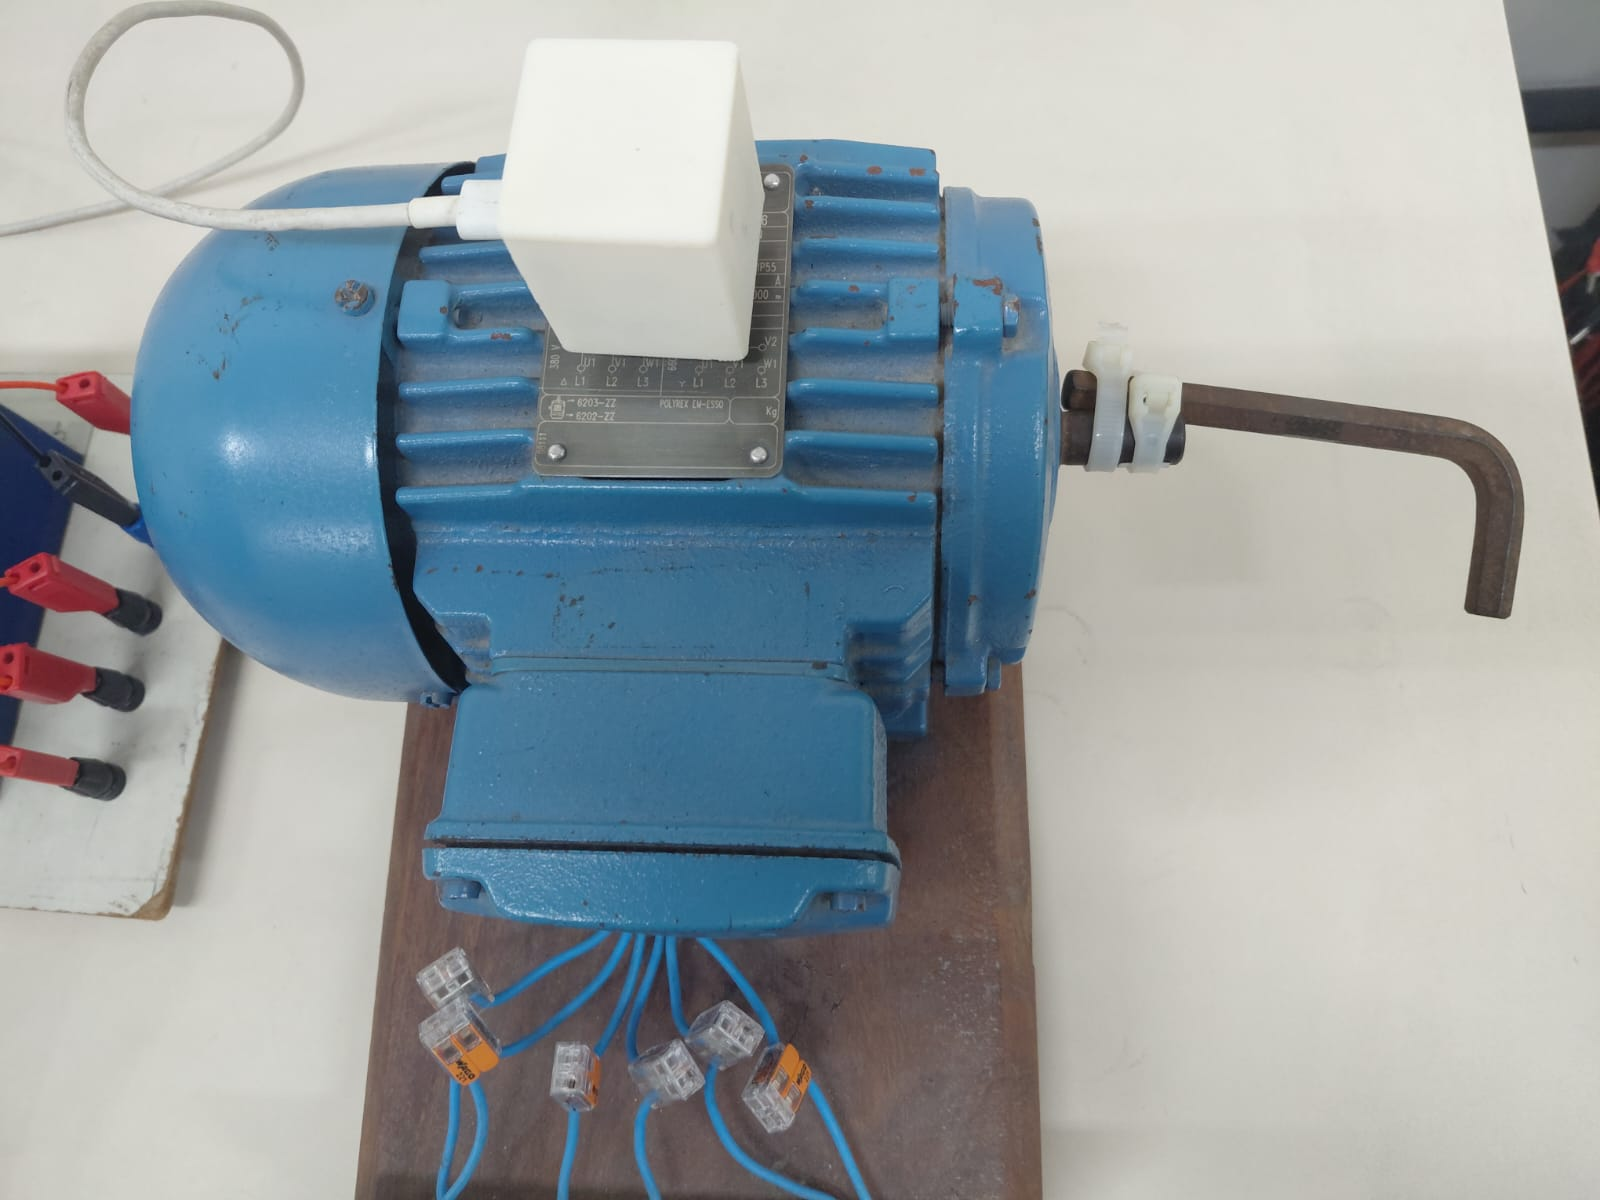
\includegraphics[width=0.5\columnwidth]{Figuras/desba_chave.jpg}
    \caption{Perturbação induzida no MIT por meio de carga desbalanceadora.}
    \label{fig:perturbacaoDesbalanceamento}
    {\footnotesize Fonte: Elaborado pelo autor.}
\end{figure}

Após o acionamento do motor novamente a 30 Hz, foi obtido o sinal de velocidade apresentado na Figura~\ref{fig:desbalanceamentoVel}. Observa-se uma alteração significativa no comportamento do sinal, especialmente no eixo $Y$, que apresenta uma característica aproximadamente senoidal. Esse comportamento indica a predominância de uma componente periódica em relação às demais componentes presentes no sinal, diferindo do comportamento observado para o motor sem a carga desbalanceadora, apresentado na Figura~\ref{fig:normal_velocidade_30}.

\begin{figure}[!ht]
    \centering
    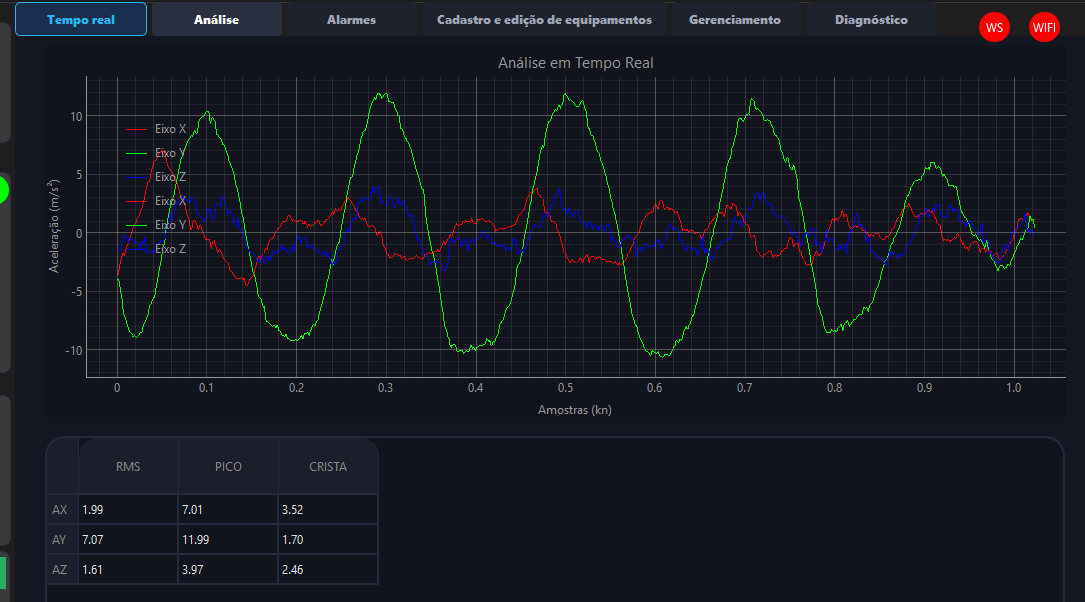
\includegraphics[width=0.95\columnwidth]{Figuras/desbalanceamento_desb_vel_30.png}
    \caption{Desbalanceamento: velocidade no domínio do tempo.}
    \label{fig:desbalanceamentoVel}
    {\footnotesize Fonte: Elaborado pelo autor.}
\end{figure}

A aplicação da FFT ao sinal de velocidade permitiu verificar essa
característica no domínio da frequência. Conforme apresentado na
Figura~\ref{fig:desbalanceamentoFFT_vel}, observa-se uma componente
predominante próxima a 15 Hz no eixo $Y$. Considerando que o motor
apresenta velocidade síncrona de 1800 rpm a 60 Hz, a operação do
inversor a 30 Hz corresponde, para as condições do ensaio, a uma
velocidade de aproximadamente 900 rpm, equivalente a uma frequência
de rotação de 15 Hz.

A presença de uma componente predominante em aproximadamente
$1\times f_{\mathrm{rot}}$, coincidente com a frequência de rotação do
eixo, é característica do comportamento vibratório associado ao
desbalanceamento. Isso ocorre porque a massa desbalanceadora produz
uma força centrífuga periódica cuja frequência de repetição é igual à
frequência de rotação do eixo. Dessa forma, o pico observado em
aproximadamente 15 Hz constitui uma evidência experimental da
condição de desbalanceamento introduzida no motor.

\begin{figure}[!ht]
    \centering
    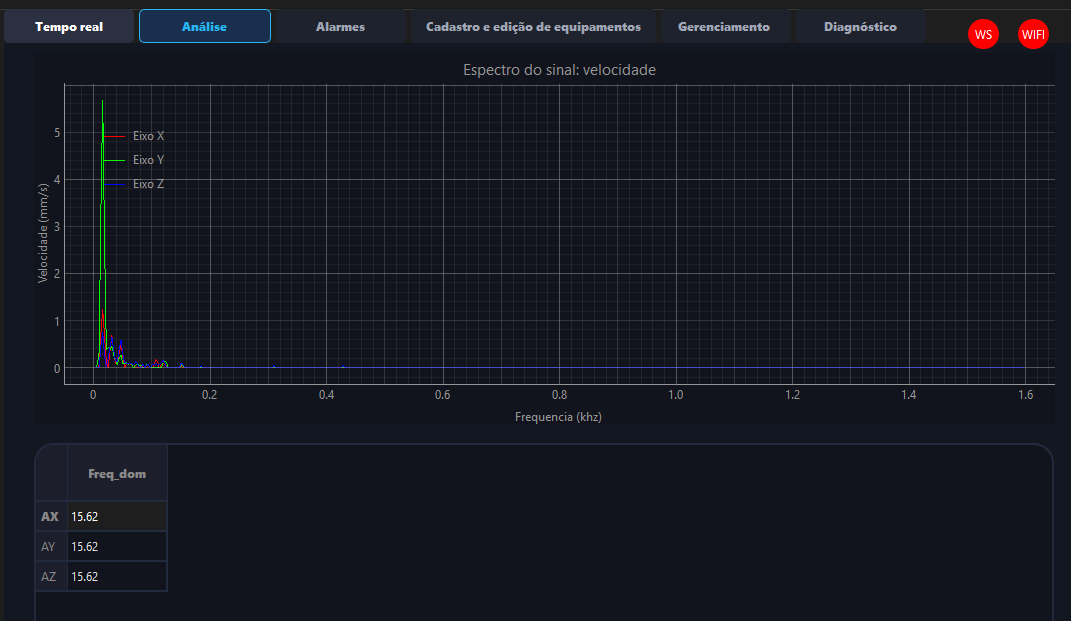
\includegraphics[width=0.95\columnwidth]{Figuras/desbalanceamento_desb_fft_30.png}
    \caption{Desbalanceamento: FFT da velocidade.}
    \label{fig:desbalanceamentoFFT_vel}
    {\footnotesize Fonte: Elaborado pelo autor.}
\end{figure}

Na análise da FFT do sinal de aceleração, apresentada na Figura~\ref{fig:desbalanceamentofft_acel}, observa-se a permanência das componentes harmônicas identificadas anteriormente na condição sem perturbação, apresentada na Figura~\ref{fig:FFT_aceleracao}. Entretanto, a presença de uma componente de elevada amplitude próxima a 15 Hz no eixo $Y$ faz com que as demais componentes apresentem menor contribuição relativa no espectro.

\begin{figure}[!ht]
    \centering
    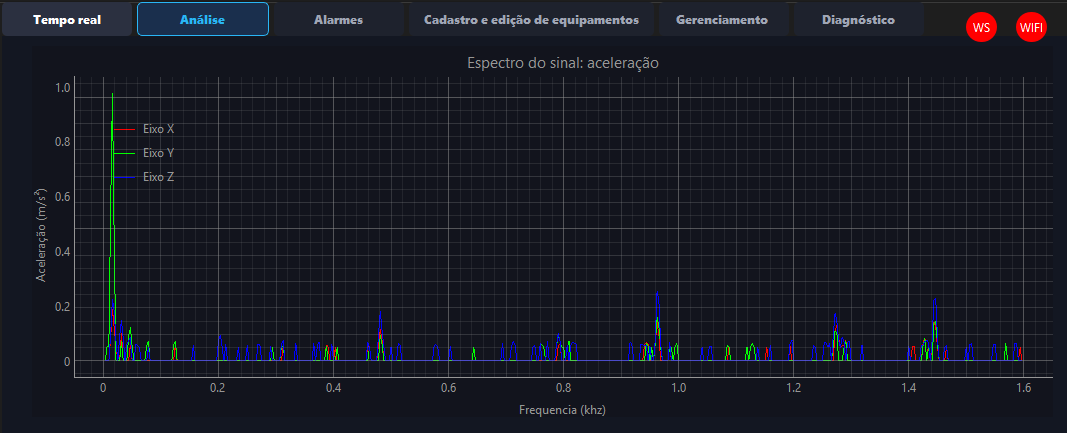
\includegraphics[width=0.95\columnwidth]{Figuras/fft_acel_30_desbalanceamento.png}
    \caption{Desbalanceamento: FFT da aceleração.}
    \label{fig:desbalanceamentofft_acel}
    {\footnotesize Fonte: Elaborado pelo autor.}
\end{figure}

A partir dessas análises, observa-se que a perturbação provocada pelo desbalanceamento está predominantemente associada às componentes de menor frequência, apresentando menor influência relativa nas componentes de frequência mais elevada. Para verificar essa característica, foi aplicada a análise do sinal envelopado por meio da transformada de Hilbert, conforme apresentado na Figura~\ref{fig:desbalanceamentohilbert}. Em comparação com o resultado obtido para a condição sem perturbação, apresentado na Figura~\ref{fig:FFT_hilbert}, observa-se comportamento espectral semelhante, indicando que a perturbação introduzida não provocou alterações significativas nas componentes de alta frequência analisadas pelo método.

\begin{figure}[!ht]
    \centering
    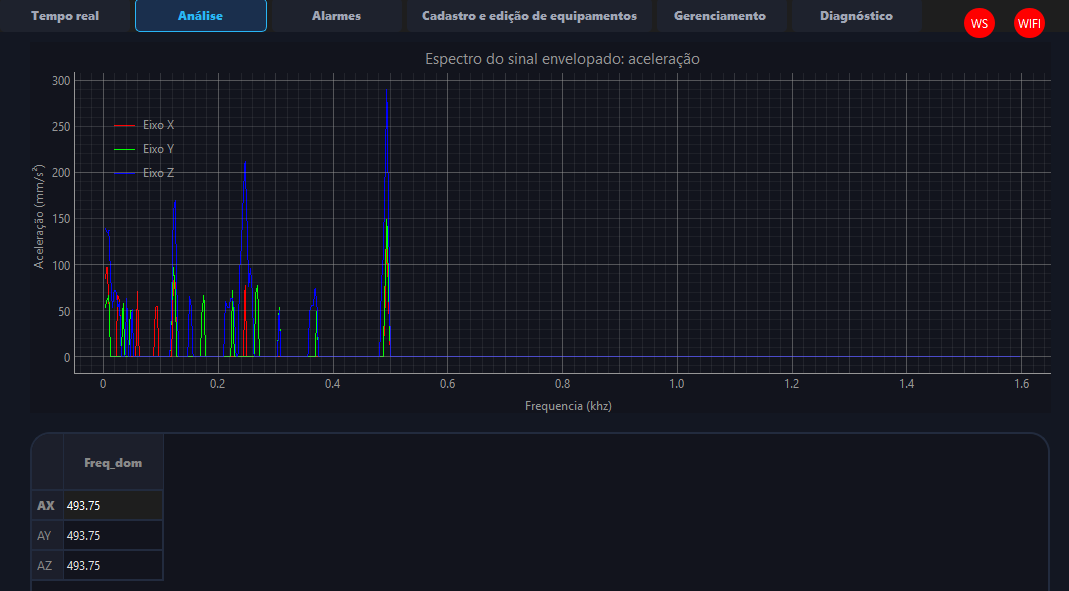
\includegraphics[width=0.95\columnwidth]{Figuras/desbalanceamento_hilbertFFT_30.png}
    \caption{Desbalanceamento: FFT do sinal envelopado.}
    \label{fig:desbalanceamentohilbert}
    {\footnotesize Fonte: Elaborado pelo autor.}
\end{figure}

Por fim, foi aplicada a transformada de wavelet ao sinal de aceleração, conforme apresentado na Figura~\ref{fig:waveletDesba}. Observa-se uma maior concentração de componentes na representação tempo-frequência, evidenciada pela presença de regiões de maior intensidade associadas à periodicidade da vibração. Esse comportamento permite visualizar a ocorrência da perturbação ao longo do intervalo de aquisição e complementa a análise realizada no domínio da frequência.

\begin{figure}[!ht]
    \centering
    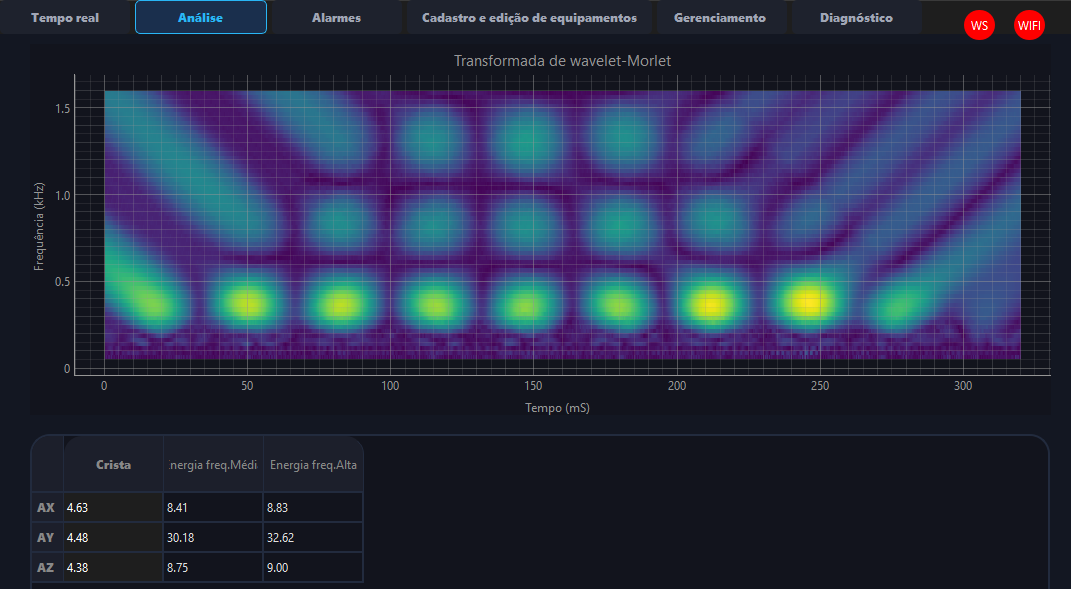
\includegraphics[width=0.95\columnwidth]{Figuras/desbalanceamento_wavelet_30.png}
    \caption{Desbalanceamento: transformada de wavelet.}
    \label{fig:waveletDesba}
    {\footnotesize Fonte: Elaborado pelo autor.}
\end{figure}

Como consequência do aumento do nível de vibração provocado pelo desbalanceamento, o sistema supervisório identificou a condição de alarme previamente configurada. O resultado apresentado pelo sistema é mostrado na Figura~\ref{fig:alarmeDesba}, demonstrando a capacidade do protótipo de detectar a alteração no comportamento vibratório e gerar o respectivo alarme.

\begin{figure}[!ht]
    \centering
    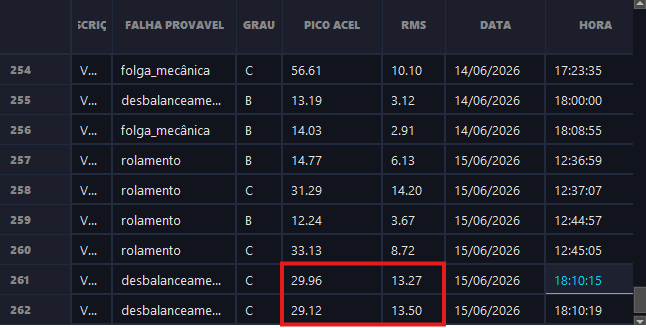
\includegraphics[width=0.95\columnwidth]{Figuras/desbalanceamentoalarmes.png}
    \caption{Alarme emitido para a condição de desbalanceamento.}
    \label{fig:alarmeDesba}
    {\footnotesize Fonte: Elaborado pelo autor.}
\end{figure}

\subsection{Análise do MIT com perturbação: impacto}

Por fim, foram realizados ensaios com impactos mecânicos aplicados ao MIT, com o objetivo de simular uma condição de folga mecânica. Devido à natureza transitória desse fenômeno, foram priorizadas análises capazes de evidenciar sua ocorrência no domínio do tempo e no domínio tempo-frequência.

No domínio do tempo, observa-se na Figura~\ref{fig:impactoVel} um pico elevado de velocidade seguido por uma resposta de amplitude decrescente até o retorno ao regime estacionário. Esse comportamento evidencia a característica transitória do impacto e sua diferença em relação à condição de operação sem perturbação.

\begin{figure}[!ht]
    \centering
    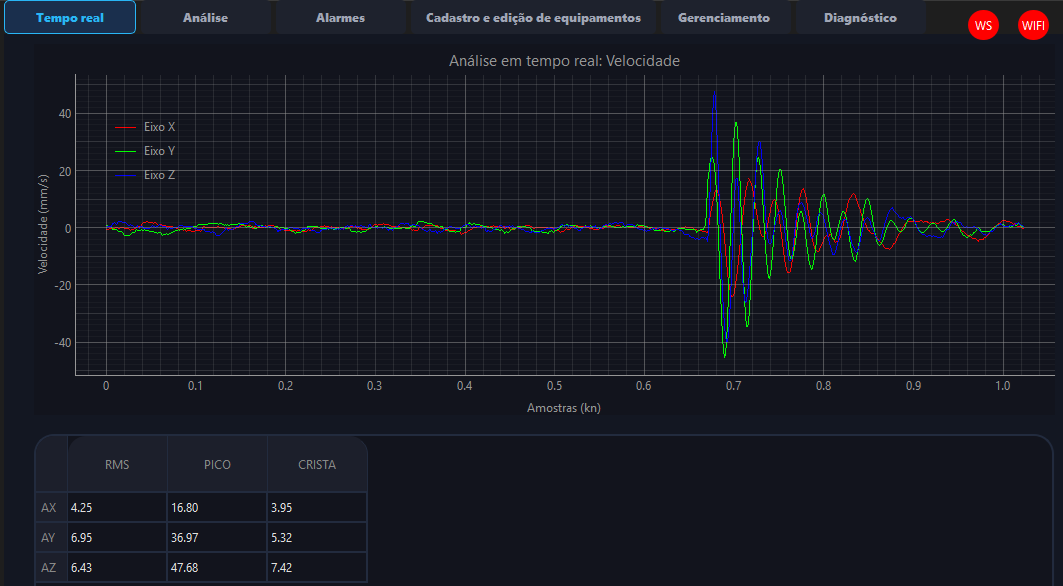
\includegraphics[width=0.95\columnwidth]{Figuras/impacto_vel.png}
    \caption{MIT com impacto: sinal de velocidade.}
    \label{fig:impactoVel}
    {\footnotesize Fonte: Elaborado pelo autor.}
\end{figure}

A FFT do sinal de velocidade, apresentada na Figura~\ref{fig:FFTimpactoVel}, evidencia a distribuição das componentes espectrais associadas ao evento transitório, com maior concentração nas baixas frequências e redução progressiva de sua contribuição.

\begin{figure}[!ht]
    \centering
    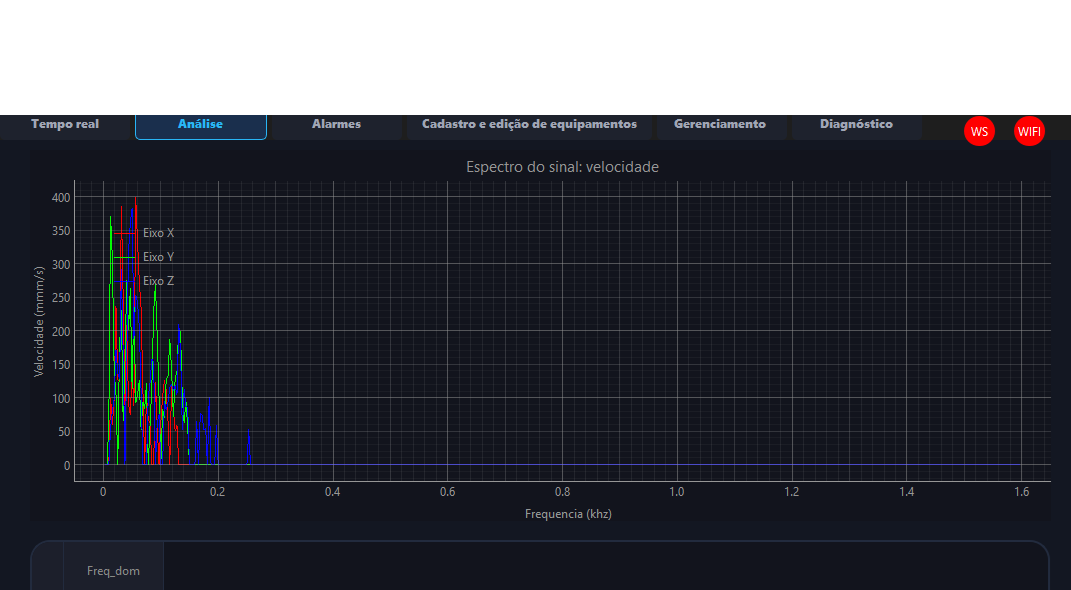
\includegraphics[width=0.95\columnwidth]{Figuras/impacto_vel_fft.png}
    \caption{MIT com impacto: FFT do sinal de velocidade.}
    \label{fig:FFTimpactoVel}
    {\footnotesize Fonte: Elaborado pelo autor.}
\end{figure}

A análise por transformada de wavelet, apresentada na Figura~\ref{fig:waveletImpacto}, permitiu localizar temporalmente o evento e identificar a faixa de frequência associada à sua ocorrência. Observa-se uma concentração de energia em torno de 100 Hz durante um intervalo curto, seguida pela redução de sua intensidade, em concordância com o comportamento transitório observado no domínio do tempo.

\begin{figure}[!ht]
    \centering
    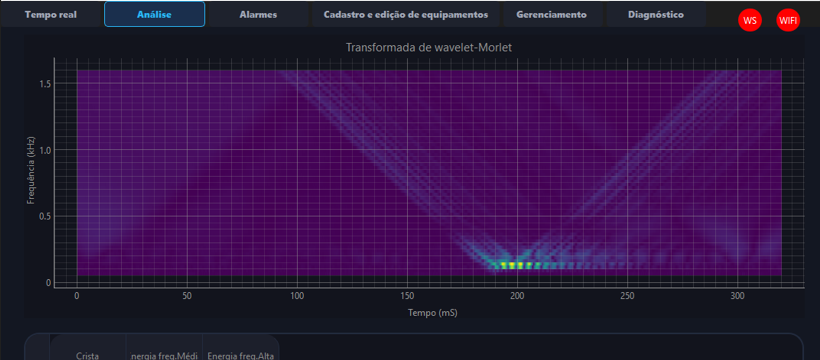
\includegraphics[width=0.95\columnwidth]{Figuras/impacto_acel_wavelet.png}
    \caption{MIT com impacto: transformada de wavelet.}
    \label{fig:waveletImpacto}
    {\footnotesize Fonte: Elaborado pelo autor.}
\end{figure}

Em um dos ensaios, o sistema supervisório classificou a ocorrência como severidade D, conforme apresentado na Figura~\ref{fig:alarmImpacto}. O resultado foi associado à ocorrência de um elevado valor de pico de velocidade, enquanto o valor RMS permaneceu relativamente baixo, característica compatível com um evento impulsivo.

\begin{figure}[!ht]
    \centering
    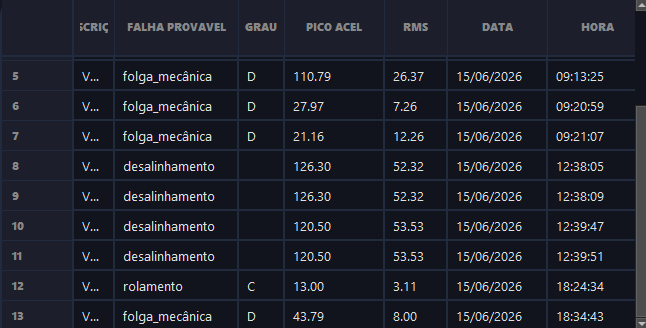
\includegraphics[width=0.95\columnwidth]{Figuras/alarmes_impacto.png}
    \caption{Alarme de severidade D associado ao impacto.}
    \label{fig:alarmImpacto}
    {\footnotesize Fonte: Elaborado pelo autor.}
\end{figure}






% Utiliza o estilo padrão exigido pela IEEE (numérico em ordem de citação)
\bibliographystyle{IEEEtran}

% Aponta para o seu arquivo .bib (substitua 'references' pelo nome do seu arquivo, sem a extensão)
\bibliography{references}


\end{document}
